\documentclass{style/CRPITStyle}
\usepackage{epsfig}   % Packages to use if you wish
\usepackage{lscape}   %
\usepackage[authoryear]{natbib}
\renewcommand{\cite}{\citep}
\pagestyle{empty}
\thispagestyle{empty}
\hyphenation{roddick}

\begin{document}

\title{Software Development: An Evaluation of KPSmart Development}
\author{David Barnett}
\affiliation{School of Engineering and Computer Science \\
Victoria University of Wellington, \\
PO Box 600, Wellington, 6140 \\
Email:~{\tt barentdavi@myvuw.ac.nz}}

\maketitle

\begin{abstract}
\end{abstract}

\vspace{.1in}

\section{Introduction}

% Which process model your team has chosen for the project and why, and
% how your team used the process model,
\section{Process Model}

%The experiences you made with using the process model and the lessons
% you learned from the project
\section{Experience}

% How well your application meets the requirements gathered during the
% initial requirements analysis and what you have done to ensure your ap-
% plication meets the requirements
\section{Requirements}

% What kind of system is your application, i.e., S-system, E-system or P-
% system and why?
\section{System Type}


\cite{lehman:1980}

\vspace{.1in}

\begin{figure}[htb]
\fbox{\parbox[b]{.99\linewidth}{
\vskip 0.5cm
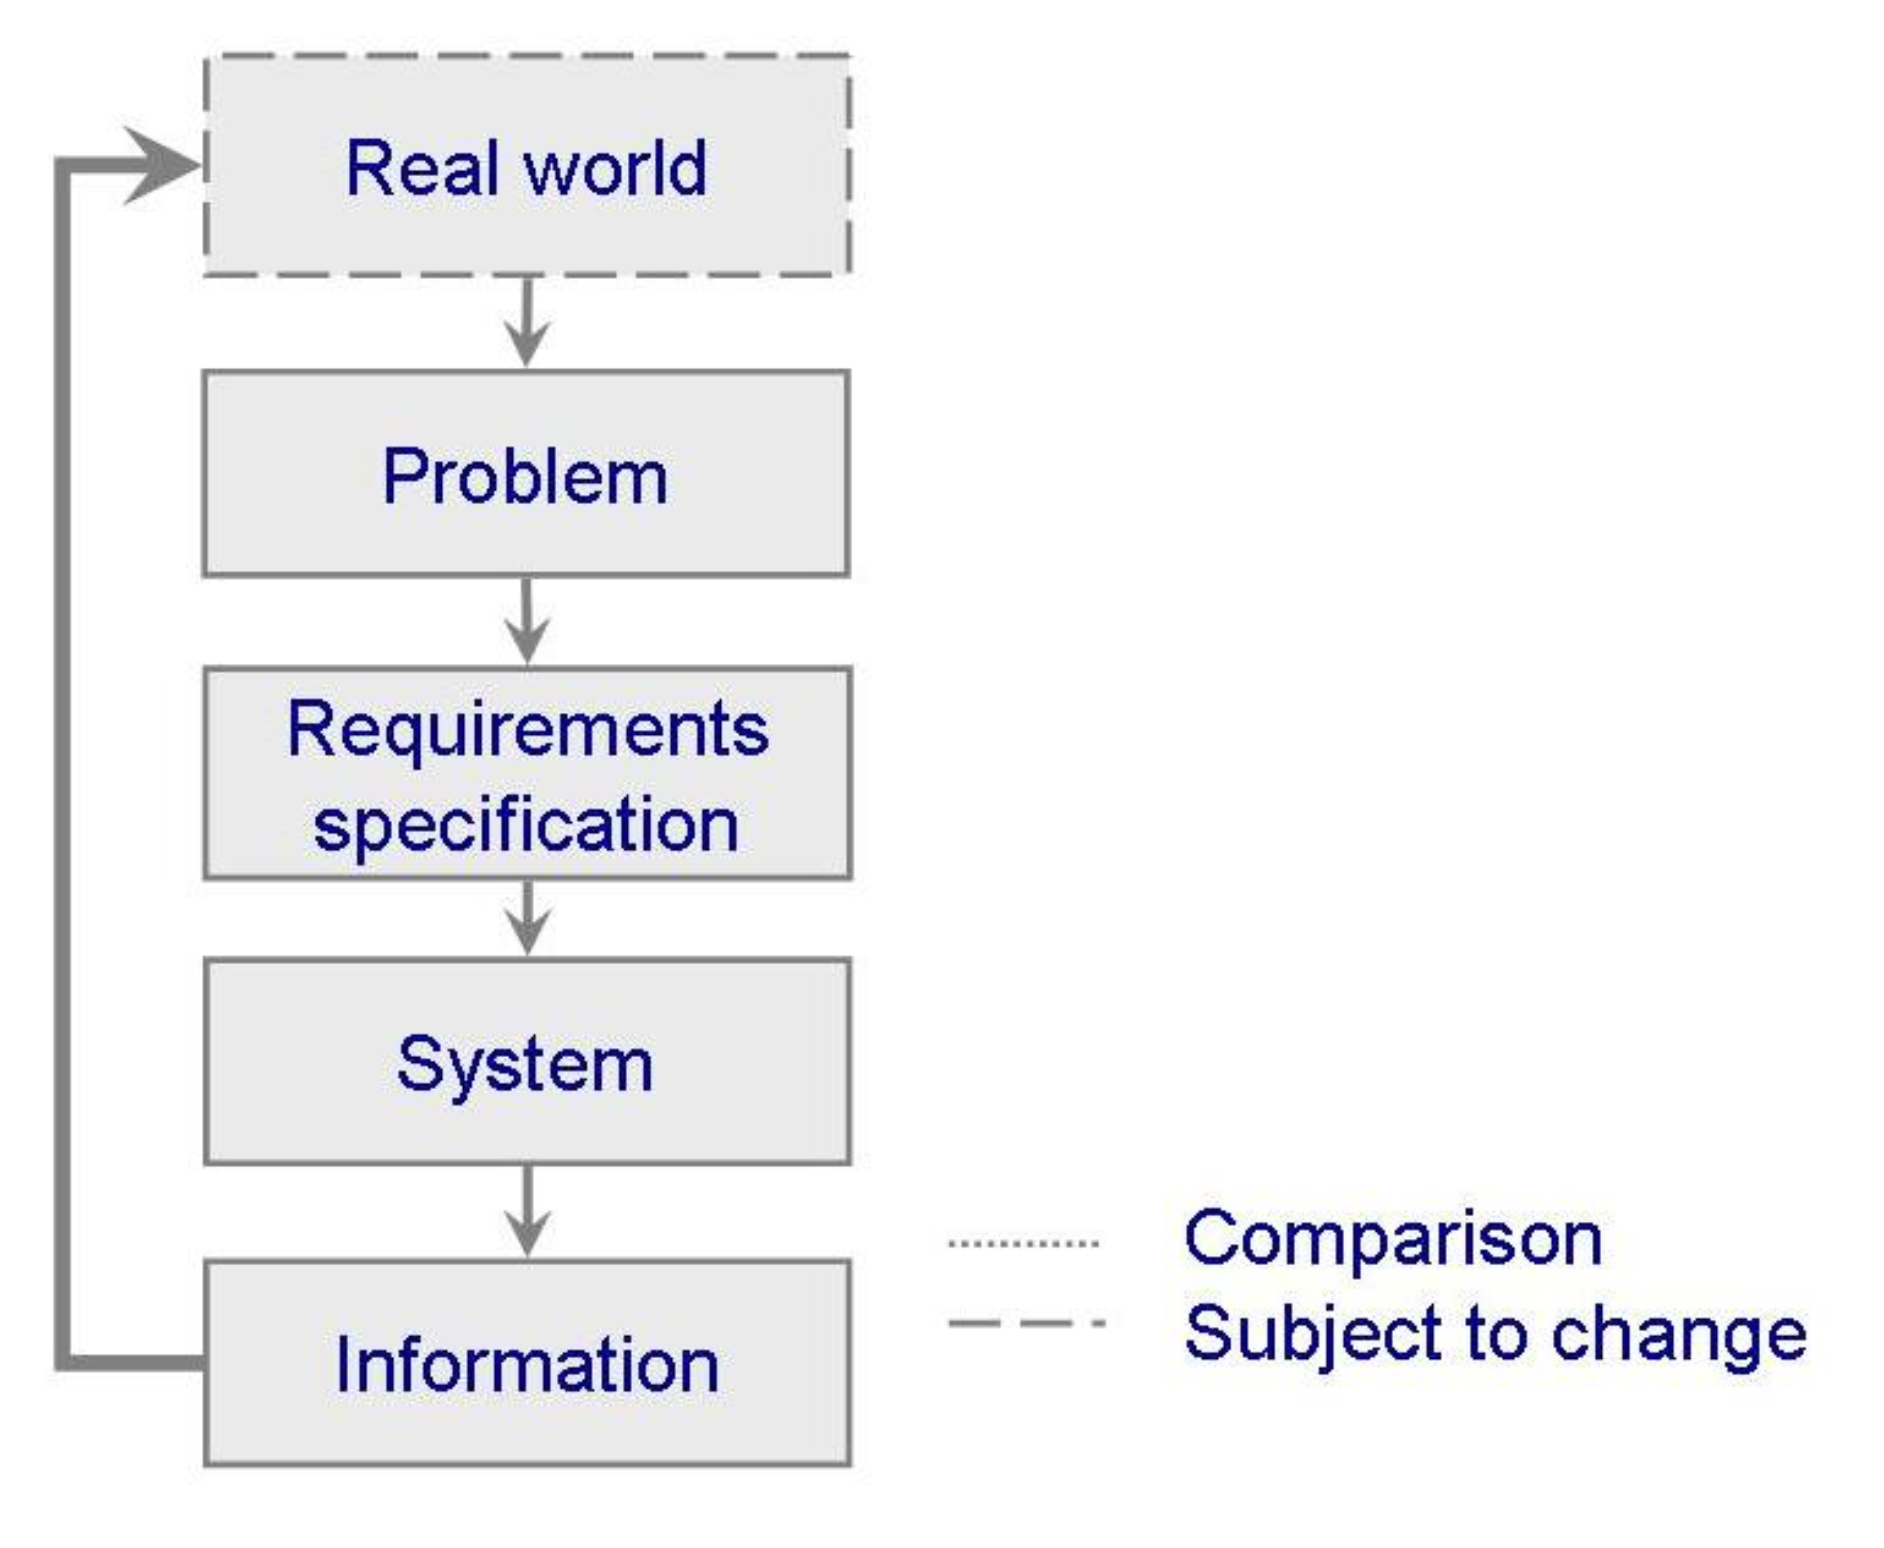
\includegraphics[width=0.45\textwidth]{figures/s-system.png}
\vskip 0.5cm}}
\caption{\protect\label{s-system}  S-System, figure by Dr. Stephen Marshall  }
\end{figure}

\vspace{.1in}

\vspace{.1in}

\begin{figure}[htb]
\fbox{\parbox[b]{.99\linewidth}{
\vskip 0.5cm
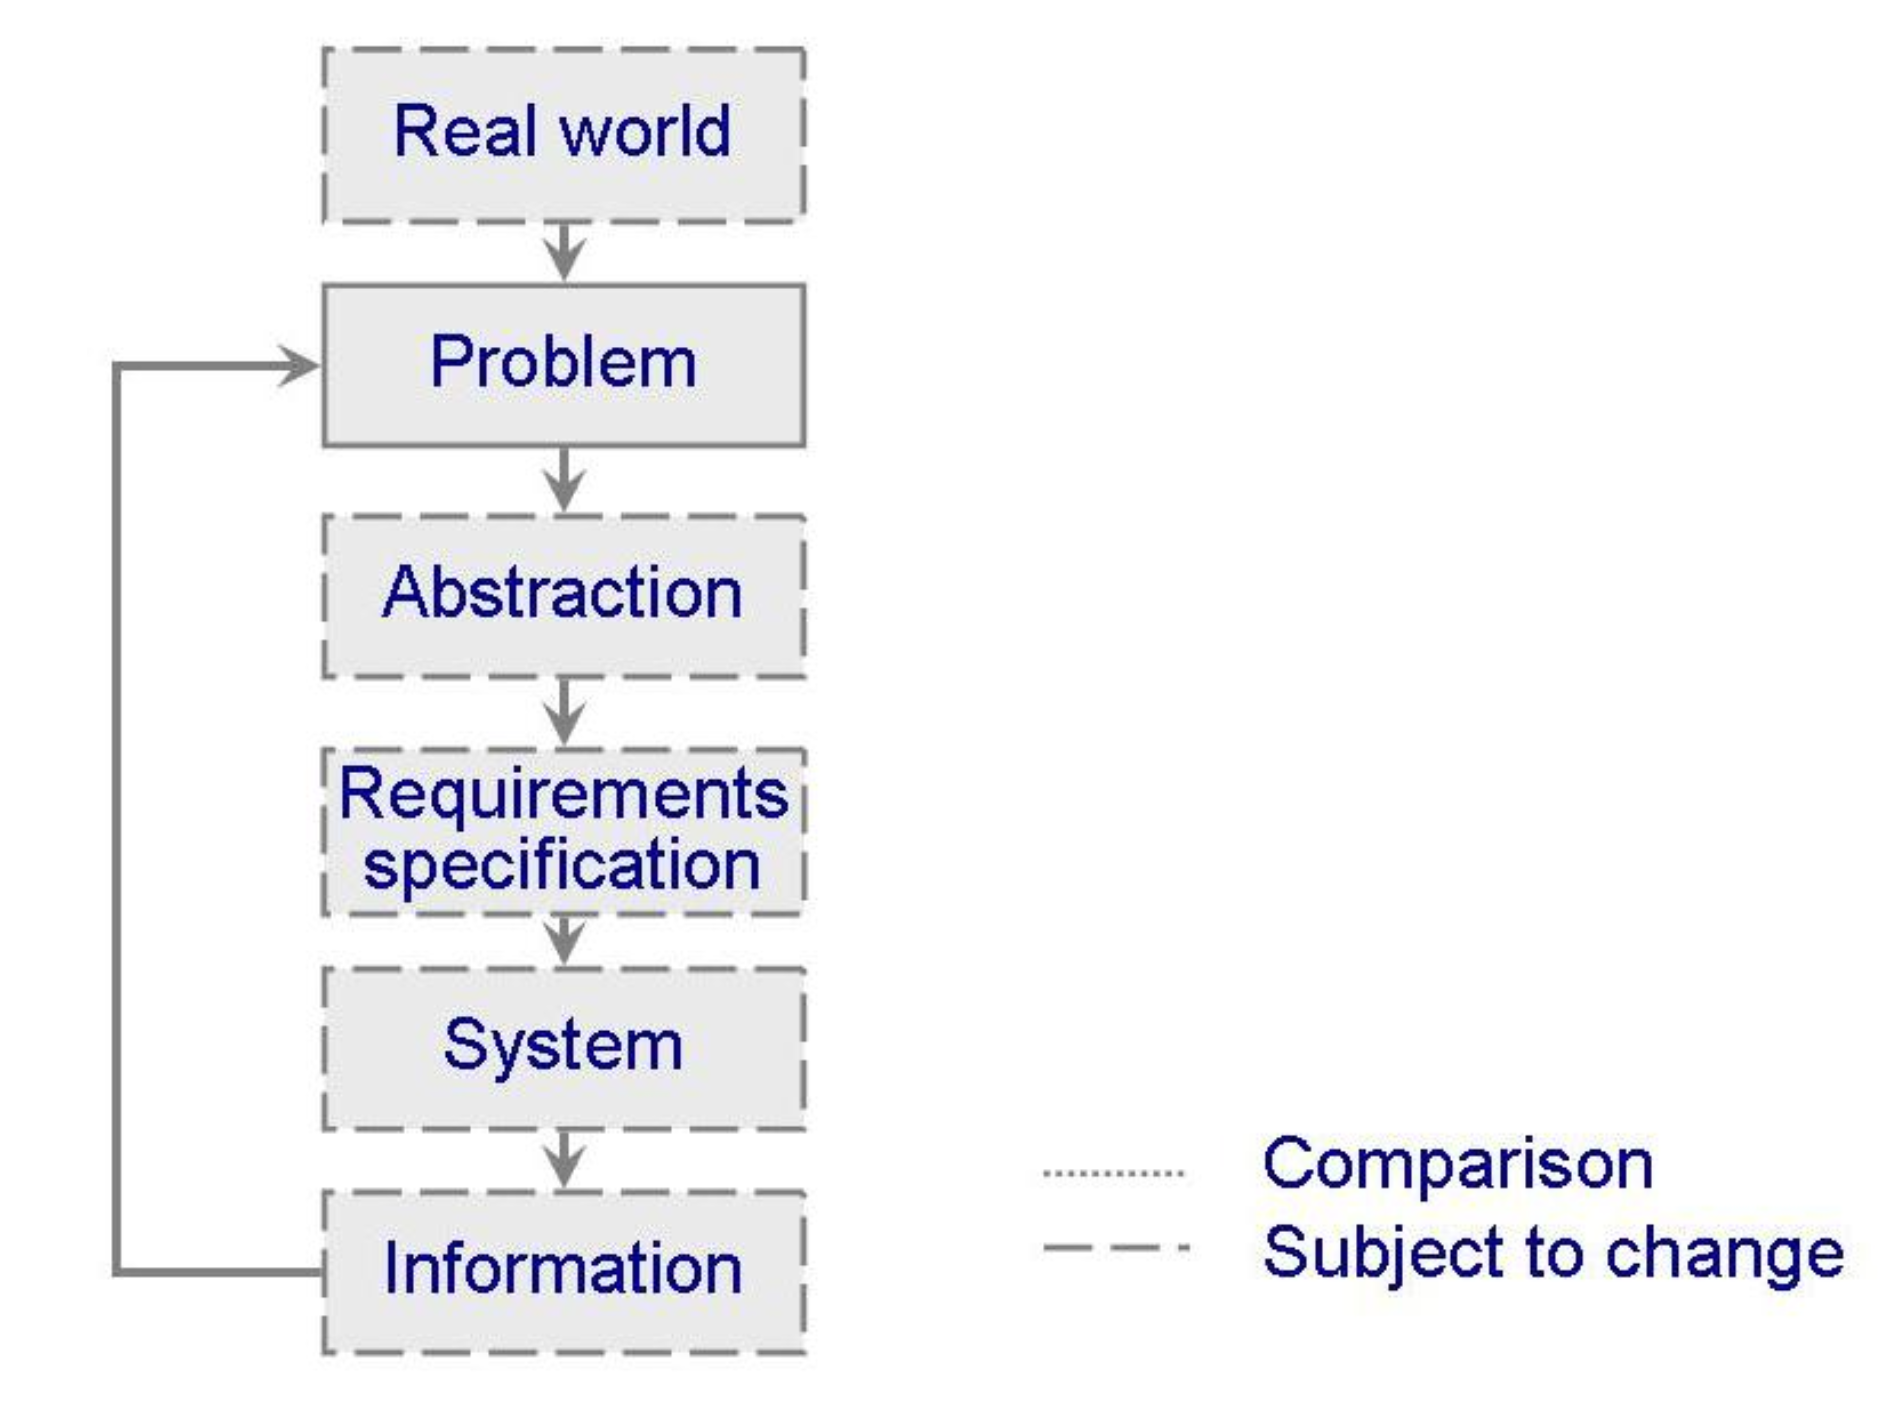
\includegraphics[width=0.45\textwidth]{figures/p-system.png}
\vskip 0.5cm}}
\caption{\protect\label{p-system}  P-System, figure by Dr. Stephen Marshall  }
\end{figure}

\vspace{.1in}

\vspace{.1in}

\begin{figure}[htb]
\fbox{\parbox[b]{.99\linewidth}{
\vskip 0.5cm
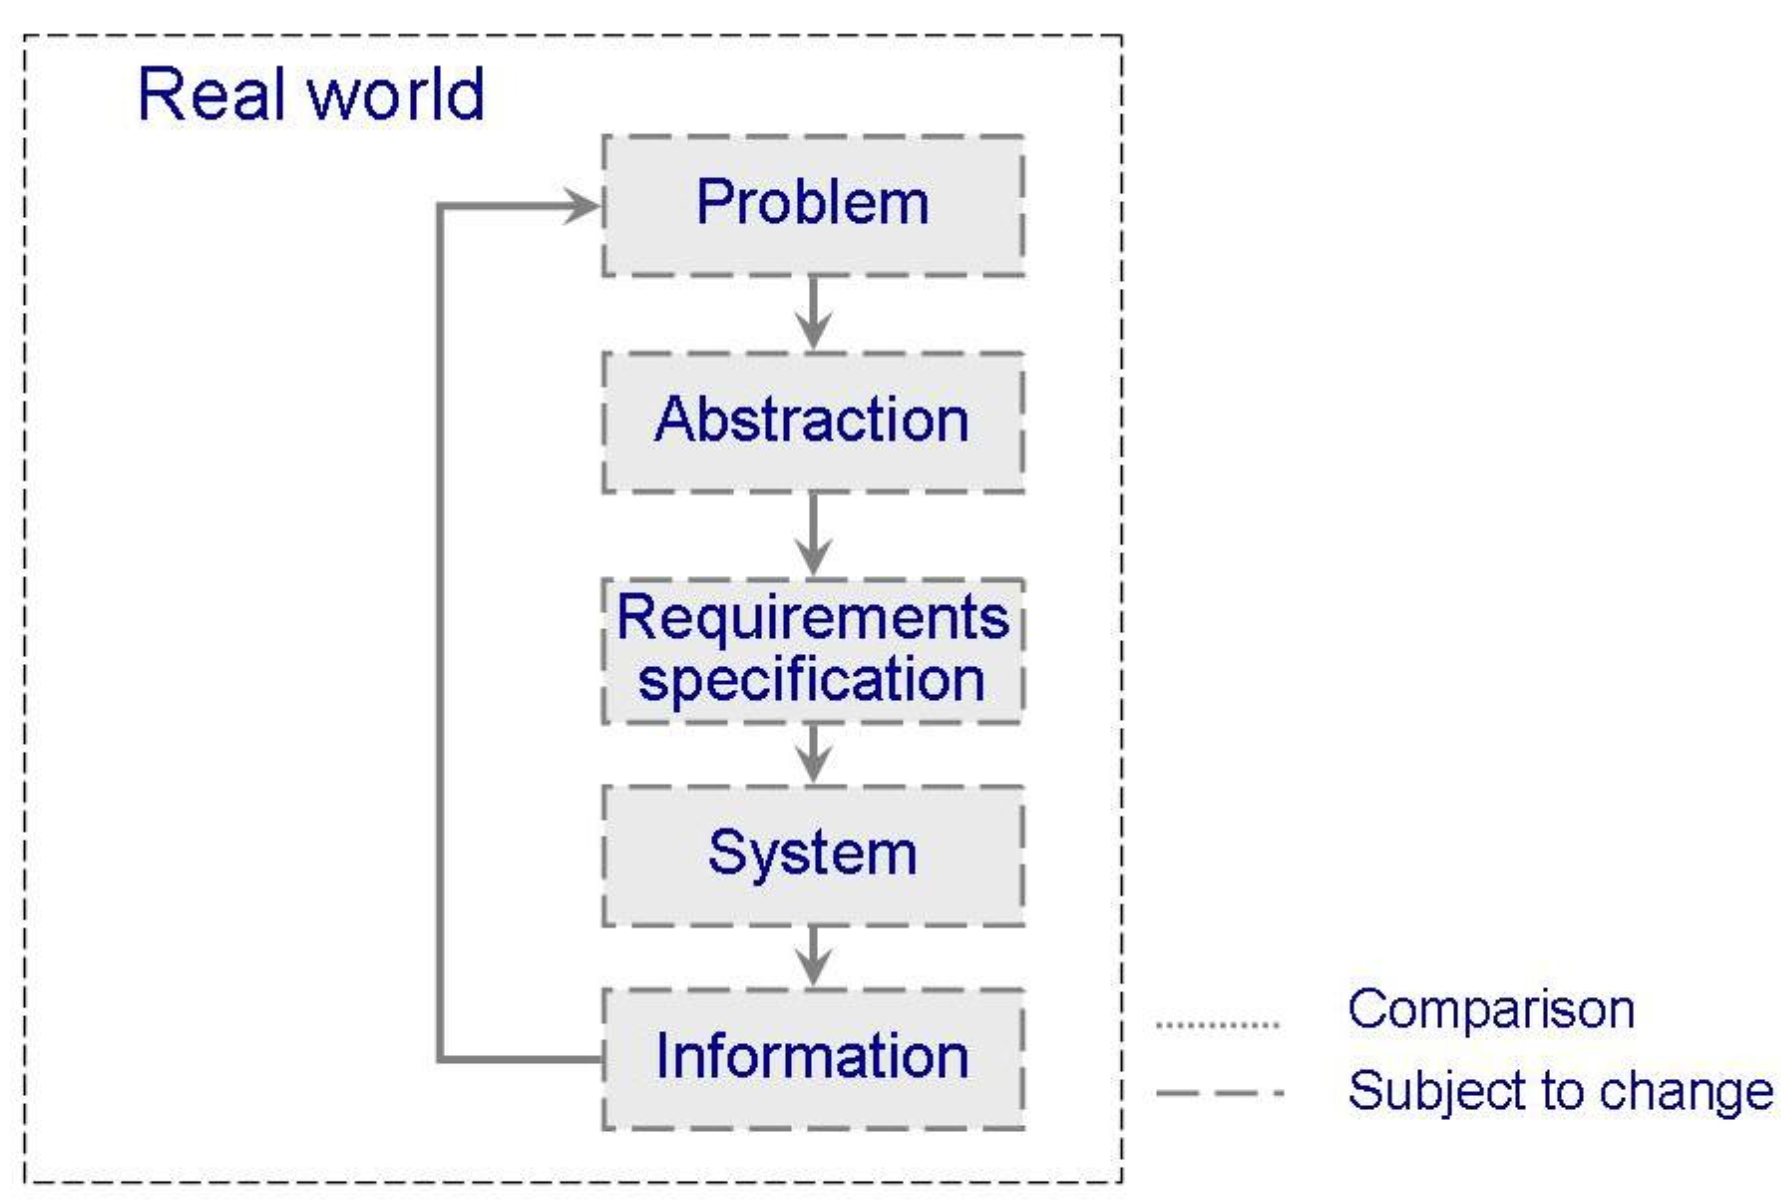
\includegraphics[width=0.45\textwidth]{figures/e-system.png}
\vskip 0.5cm}}
\caption{\protect\label{e-system}  E-System, figure by Dr. Stephen Marshall  }
\end{figure}

\vspace{.1in}

% What kind of maintenance activities may be needed to maintain the ap-
% plication. Recall that four types of software maintenance activities were
% discussed in the lectures.
\section{Maintenance}

% What process model would you use if the project were developed as an
% open source application, and why?  Which Indirect Sale-Value model,
% discussed in the lecture, can be used for your application, and how?
\section{Open source}

\cite{raymond:1999}

\section{Conclusion}

\bibliographystyle{agsm}
\bibliography{report}

\end{document}

% vim:set spell et sw=4 ts=4 tw=80:
